\section{Performance and Bechmarking}
\label{Chapter:Performance}

\subsection{Characterization}
An important aspect of fabricating a new technique is measuring how well it performs in different usage scenarios. Developing metrics for judging the artistic quality of a calligraphy specimen produced by the bezier or rotating bezier splines is altogether a separate discussion and out of scope of this research. However, there are some aspects that we have tried to measure the effectiveness of the rotating splines.

\subsection{Supported Script}
All the scripts we analyzed are written with rigid broad-edge tools, such as broad-edge pens and markers, where the tool keeps complete contact with the surface throughout the stoke. However, if the script requires changing the extent of tool contact with the surface, the best alternate to achieve a similar appearance of the script would be to use multiple splines with multiple thicknesses that overlap each other in a gradual manner. The rotating bezier splines cannot control the tool inclination and applied pressure, therefore, they are not suitable for scripts written with flexible tools like broad-edge brushes.

\subsubsection{Coverage}
To benchmark the performance and accuracy of rotating bezier splines, some test results are presented here. These values are produced by comparing high resolution binary images of actual scripts, extracted with Adobe Photoshop and rasterized images produced by the twisting bezier splines originally formed by tracing the processed images. The pixel density is set such that a pixel-pixel comparison can be performed between the original image and the rasterized splines. The accuracy is analysed by computing the overflow and underflow of the ink by matching pixels of both images. Table \ref{Table:Accuracy} shows a summary of these benchmark results.

\begin{table}
\begin{center}
\caption{Benchmark of the mathematical accuracy of the twisting bezier spline curves}
\label{Table:Accuracy}
\begin{tabular}{| c | c |}
  \hline
\textbf{Metrics} & \textbf{Results} \\
  \hline
Area over flow & $<$ 2\% \\
  \hline
Coverage & $>$ $94\%$ \\
  \hline
Lateral deviation from the pitch line & N.A. \\
  \hline
Compatibility & All broad edge scripts \\
  \hline
Total splines measured & $>100$ \\
  \hline
Total pixels compared & $9.9$~million \\
  \hline
Tested scripts & Nastaleeq, Thuluth \\
\hline
\end{tabular}
\end{center}
\end{table}
%
%This metrics is comprehensive but still not complete. Some additional metrices are still needed to give a verdict about how good the proposed solution is and it is now up to the community to evolve these curves according to the needs. Table \ref{Table:AdvancedMetrices} presents a couple of those metrices that may also be desired by the researchers.
%
%\begin{table}
%\begin{center}
%\caption{Advanced metrices to gauge the effectiveness of twisting bezier splines.}
%\label{Table:AdvancedMetrices}
%\begin{tabular}{| c | c |}
%  \hline
%  \textbf{Metrics} & \textbf{How can it be measured} \\
%  \hline
%Easy of usage & A survey based on Likert scale \\
%  \hline
%Time efficiency of tracing & Comparison of the time taken by the same artists tracing with conventional and rotating bezier splines \\
%  \hline
%The artistic quality of the specimens produces. & A survey based on Likert scale and filled by a wide range of artists \\
%  \hline
%\end{tabular}
%\end{center}
%\end{table}

% Please note that the third metrics in Table \ref{Table:AdvancedMetrices} seems potent for gauging the performance of atypical supline but is no longer valid given the nature of fabricated splines.

\subsubsection{Sample Results}
As both a test and a tribute, two scripts by the famous teacher, artist and author of $18$ calligraphy books, late Khursheed Gohar Qalam \cite{bib23} of the National College of Arts (NCA) were borrowed; one in Nastaleeq style and other in Thuluth. Figure \ref{Fig:Nastaleeq} and Figure \ref{Fig:Thuluth} show the bezier spline sets created by tracing both scripts respectively. Figure \ref{Fig:Nastaleeq}(a) and Figure \ref{Fig:Thuluth}(a) show the images of both script samples. Figure \ref{Fig:Nastaleeq}(b) and \ref{Fig:Thuluth}(b) are the rotating splines created by manually tracing the originals. Figure \ref{Fig:Nastaleeq}(c) and \ref{Fig:Thuluth}(c) highlight individual overlapping spline strokes. Table \ref{Table:Accuracy} shows a quantitative measure of accuracy for these script traces.

It must also be noted that since the original script image is not available in a sufficiently high digital quality, the digitization and preprocessing error also contributes to the final error in under and over flow of the rotating bezier splines.

    \begin{figure}[!t]
    \centering
    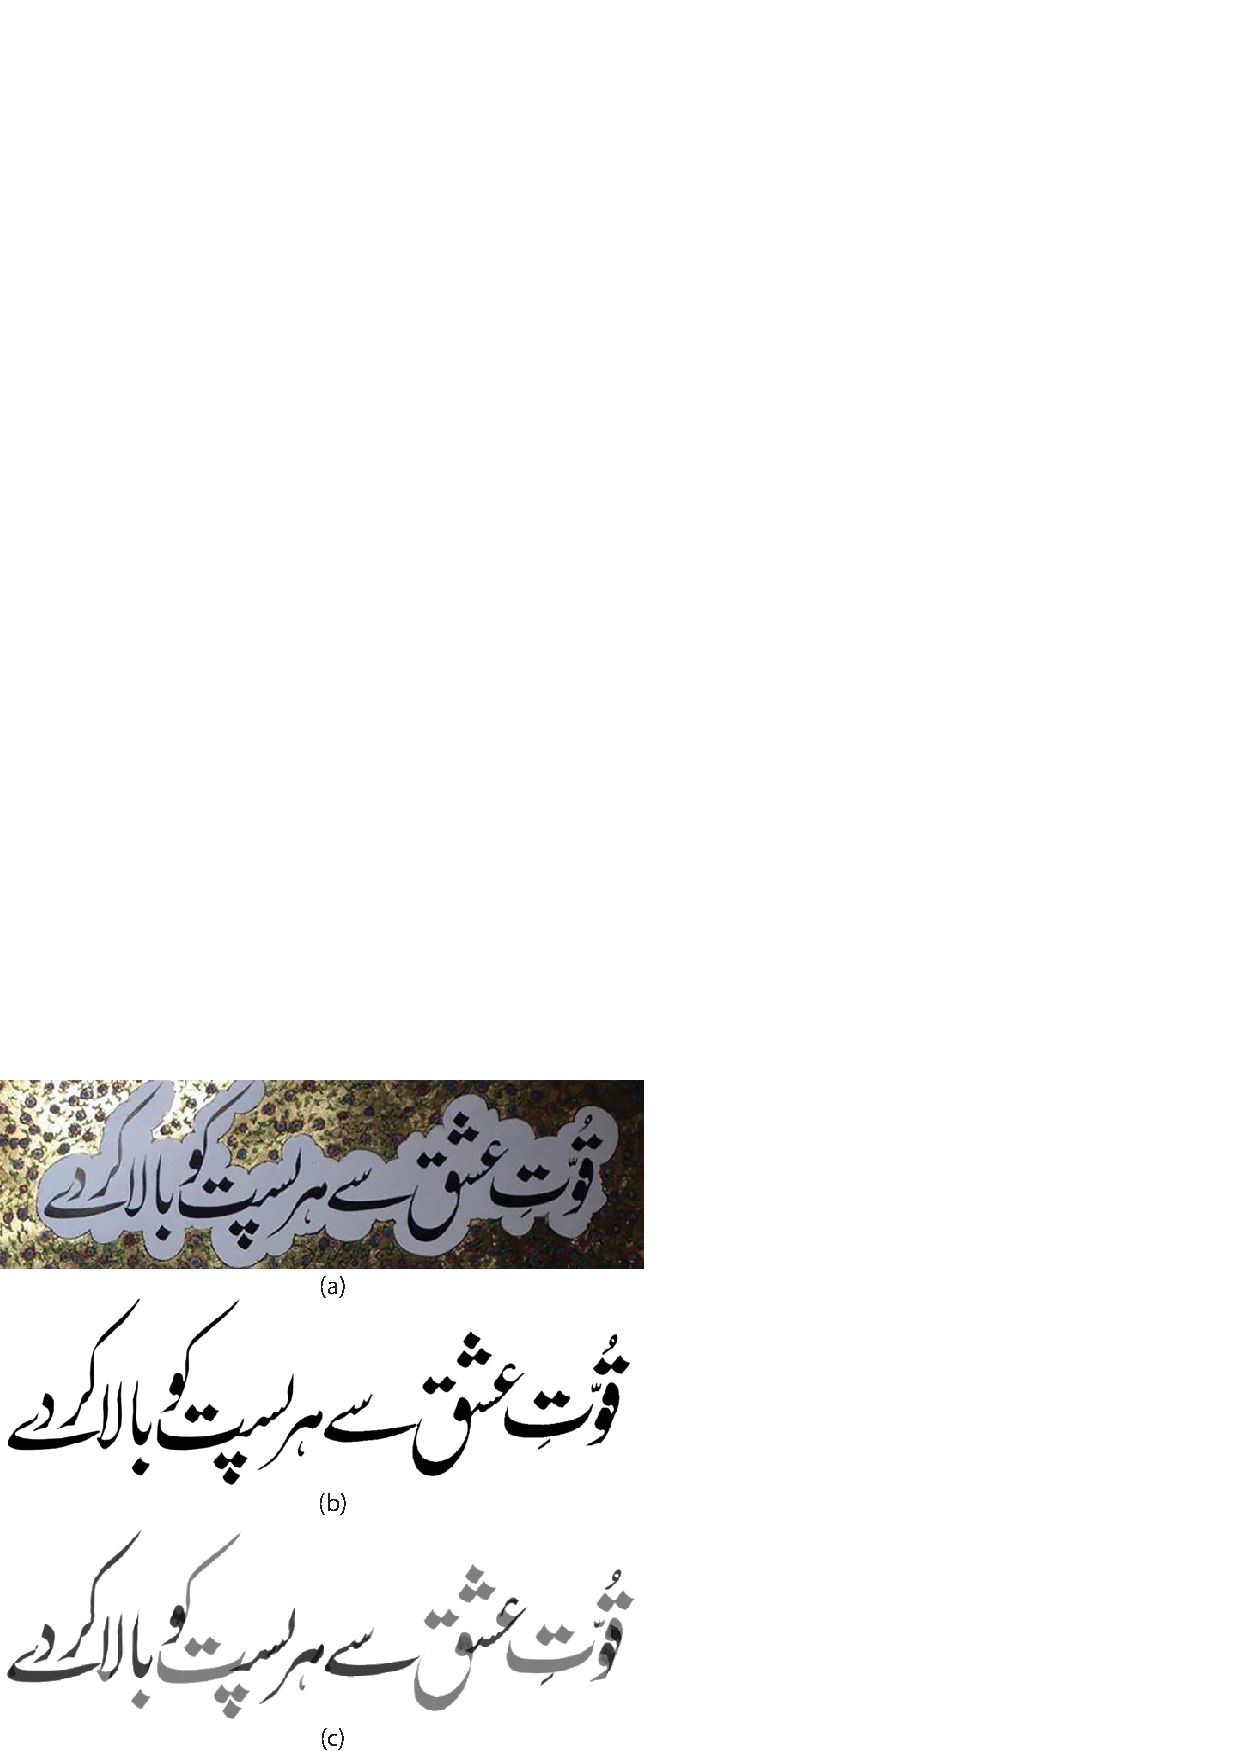
\includegraphics[width=2.5in]{../Images/NastaleeqSample.pdf}
      \caption{
        A specimen produced in ``Nastaleeq'' script. (a) Original photograph of the specimen (b) Rasterized binary image of the twisting spline curves. (c) Rasteriezd shaded image of the twisting spline curves highlighting individual curve parts.}
      \label{Fig:Nastaleeq}
    \end{figure}


    \begin{figure}[!t]
    \centering
    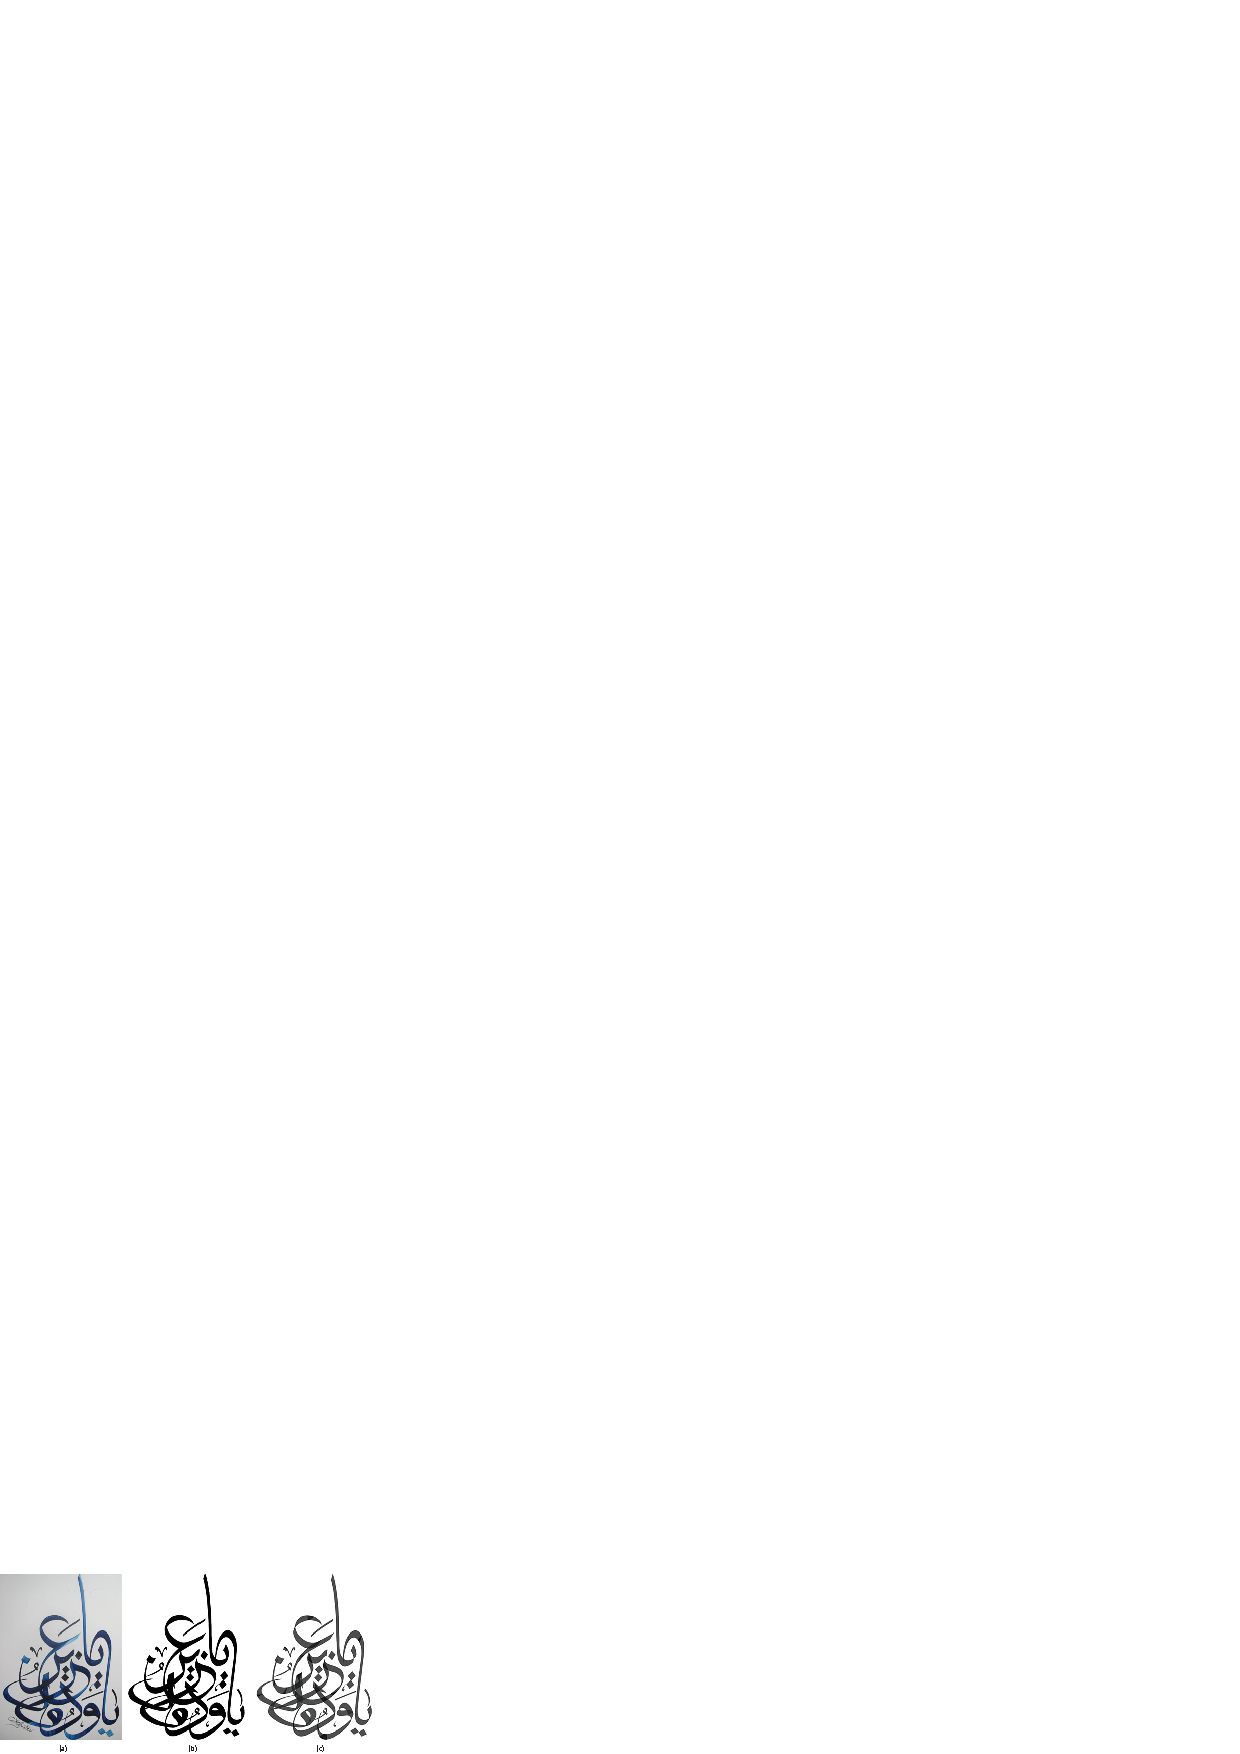
\includegraphics[width=2.5in]{../Images/ThuluthSample.pdf}
    \caption{
        A specimen produced in ``Thuluth'' script. (a) Original photograph of the specimen (b) Rasterized binary image of the twisting spline curves. (c) Rasteriezd shaded image of the twisting spline curves highlighting individual curve parts.
    }
  \label{Fig:Thuluth}
\end{figure}

\section{Machine Data Generation and Robotic Simulation}
\label{Chapter:Simulation}
    To check how accurately the data generated by these splines can be traced by an actual robotic manipulator, a computer simulation was used. We developed an open-source simulator and tailored it for the task. The simulator assumes an open loop robot composed of six rotary joints attached in series and all powered by stepper motors with controllable step size.

\subsection{Data Generation}
    To generate machine data, the simulator first rasterizes the whole spline such that the distance between two adjacent points is always smaller than the desired linear resolution. This is done by minimizing the error between the required resolution and the linear distance between two consecutive point. For a particular point $P_N$ according to the spline model (equations \ref{splineModel01}-\ref{splineModel04}), the error between its distance from $N - 1$ and the desired linear resolution is minimized by iterating the fraction $f$ that defines $P_N$. Once a reasonable value of $f$ is found, the program then calculates the twist component at this $f$. Once $f$ has been iterated through $[0,1]$, and the whole spline has been rastereized, the program transforms this rasterized curve onto an emulated flat writing surface placed in a user defined position and orientation. Each point results in three dimensional position and orientation which can be fed to the robot as an end-effector target.

    To switch from one spline to the other, the program also adds some additional target points in the array of these points that will lift the tool normally upwards from the writing surface for a reasonable distance. Finally, the simulator tries to travel on this array of points at a constant speed.
\subsection{Accuracy Analysis}
    While following the planned trajectory, whenever the end effector is moving close to the emulated writing pad, the projection of end-effector's flat tip onto the writing surface is continuously captured to form a discrete region which simulates the ink-mark. This two dimensional projection is extracted by the simulator to be analysed with the original source images using pixel-to-pixel comparison. The results of such a comparison can be seen in Table \ref{Table:MachineDataMetrices} which reveals the machined ink-mark has a similar degree of accuracy as compared with the original twisting bezier splines.

    \begin{table}
    \begin{center}
    \caption{Benchmark of the mathematical accuracy of the twisting bezier spline curves with a simulated manipulator}
    \label{Table:MachineDataMetrices}
    \begin{tabular}{| c | c | c | c |}
    \hline
      & \textbf{Reference} & \textbf{Coverage} & \textbf{Extra} \\
      \hline
      \multicolumn{4}{|l|}{\textbf{Nastaleeq}}\\
      \hline
      Rotating bezier spline & Original Image & 95.8\% & 5.4\% \\
      \hline
      Machined Output & Original Image & 96.7\% & 7.0\% \\
      \hline
      Machined Output & Rasterized Image & 96.7\% & 4.3\% \\
      \hline
      \multicolumn{4}{|l|}{\textbf{Thuluth}}\\
      \hline
      Rotating bezier spline & Original Image & 93.4\% & 2.8\% \\
      \hline
      Machined Output & Original Image & 95.0\% & 3.4\% \\
      \hline
      Machined Output & Rasterized Image & 97.8\% & 4.4\% \\
    \hline
    \end{tabular}
    \end{center}
    \end{table} 